\documentclass{article}
\usepackage{tikz}
\usetikzlibrary{intersections,positioning,calc}
\begin{document}

% print a point given by two coordinates in pt (output is in cm)
\newcommand*\printpoint[2]{(%
    \pgfmathparse{0.03514598035*#1}\pgfmathprintnumber{\pgfmathresult}, %
    \pgfmathparse{0.03514598035*#2}\pgfmathprintnumber{\pgfmathresult})%
}

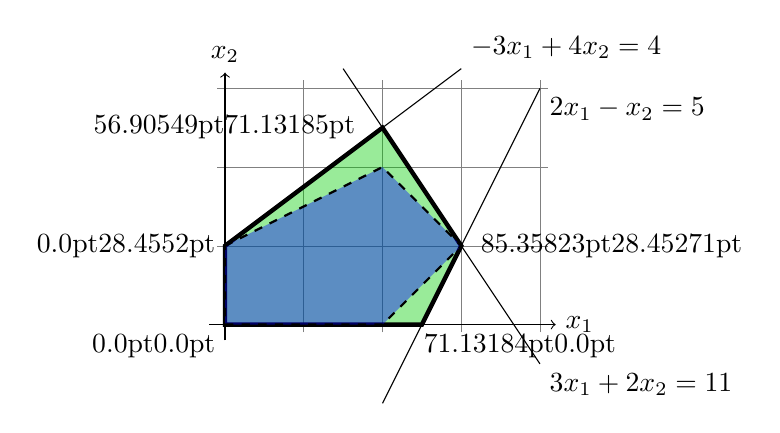
\begin{tikzpicture}
    % grid and axes
    \draw[very thin,color=gray] (-0.1,-0.1) grid (4.1,3.1);    
    \draw[->,name path=xaxis] (-0.2,0) -- (4.2,0) node[right] {$x_1$};
    \draw[->,name path=yaxis] (0,-0.2) -- (0,3.2) node[above] {$x_2$};

    % lines  
    \draw[name path=line1,domain=0:3] plot (\x,{1+ 0.75 * \x}) node[above right] {$-3x_1+4x_2 =4$};
    \draw[name path=line2,domain=1.5:4] plot (\x,{5.5 - 1.5 * \x}) node[below right] {$3x_1 + 2x_2 = 11$};
    \draw[name path=line3,domain=2:4] plot (\x,{-5+2 * \x}) node[below right] {$2x_1 - x_2 =5$}; 

    % calculate intersection points
    \node[name intersections={of=line1 and line2}] (a) at (intersection-1) {};
    \node[name intersections={of=line2 and line3}] (b) at (intersection-1) {};
    \node[name intersections={of=line3 and xaxis}] (c) at (intersection-1) {};
    \node (d) at (0,0) {};
    \node[name intersections={of=yaxis and line1}] (e) at (intersection-1) {};

    % draw the big polygon    
    \filldraw[ultra thick,fill=green!80!black,fill opacity=0.4] (a.center) -- (b.center) -- (c.center) -- (d.center)  -- (e.center) -- cycle;

    % label the vertices
    \path let \p0 = (a) in node [left=0.1cm of a] {\printpoint{\x0}{\y0}};
    \path let \p0 = (b) in node [right=0cm of b] {\printpoint{\x0}{\y0}};
    \path let \p0 = (c) in node [below right=0cm and -0.1cm of c.center] {\printpoint{\x0}{\y0}};
    \path let \p0 = (d) in node [below left=0cm of d.center] {\printpoint{\x0}{\y0}};
    \path let \p0 = (e) in node [left=0cm of e.center] {\printpoint{\x0}{\y0}};

    % draw the small polygon   
    \filldraw[thick,dashed,fill=blue,fill opacity=0.4] (0,1) -- (2,2) -- (3,1) -- (2,0) -- (0,0) -- cycle; 

\end{tikzpicture}


\end{document}
